%!TEX root = ../main.tex

\section{Comparison with previous measurements of \texorpdfstring{$\sintwobetaoreff$}{sin2beta(eff)}}
\label{sec:discussion:sin2betahistory}

Measurements of \CP violation in \BdToJPsiKS decays have been performed since
the end of the nineties. The first results by OPAL~\cite{OPAL_sin2beta},
ALEPH~\cite{ALEPH_sin2beta} and CDF~\cite{CDF_sin2beta} had an uncertainty on
\sintwobeta no better than \num{\pm0.4}. One of the main purposes of the
$B$-factories was to improve the precision, which succeeded with results of
$\SJpsiKS = \num[parse-numbers=false]{0.657\pm0.036\pm0.012}$ by
\babar~\cite{BaBar_sin2beta} and $\SJpsiKS =
\num[parse-numbers=false]{0.670\pm0.029\pm0.013}$ by
\belle~\cite{Belle_sin2beta}. Averaging the results of the $B$-factories and
combining them with measurements in various other charmonium modes leads to an
average of \sintwobeta = \num{0.679\pm0.020}~\cite{HFAG}. The measurement
presented in this thesis, using data corresponding to an integrated luminosity
of \SI{3}{\invfb} collected with the \lhcb experiment, further improves on
this yielding an updated world average of \sintwobeta =
\num{0.691\pm0.017}~\cite{HFAG}. There is also the possibility to constrain
$\beta$ from a global fit to the CKM triangle. When not using the inputs from
the direct measurements described above ($\beta =
\SI{21.85\pm0.7}{\degrees}$), a value of $\beta = (24.3
^{+1.3}_{-1.4})\,\degrees$~\cite{CKMfitter} is found. This shows that the
value found by \lhcb improves the compatibility between the direct and the
indirect measurements by shifting \sintwobeta slightly upwards.

While for \BdToJPsiKS decays mainly the value of \SJpsiKS is interesting, as
it is expected to correspond to \sintwobeta with only small corrections, the
same does not apply for the measurement of \CP violation using \BdToDD decays.
Both observables, \SDD and \CDD, have to be considered simultaneously for a
proper interpretation of the results. In \cref{fig:discussion:b2ddcomparison}
the latest results from \babar, \belle, and \lhcb, as well as the average of
these three are plotted in the two-dimensional plane of \CDD versus \SDD.
\begin{figure}[htb]
\centering
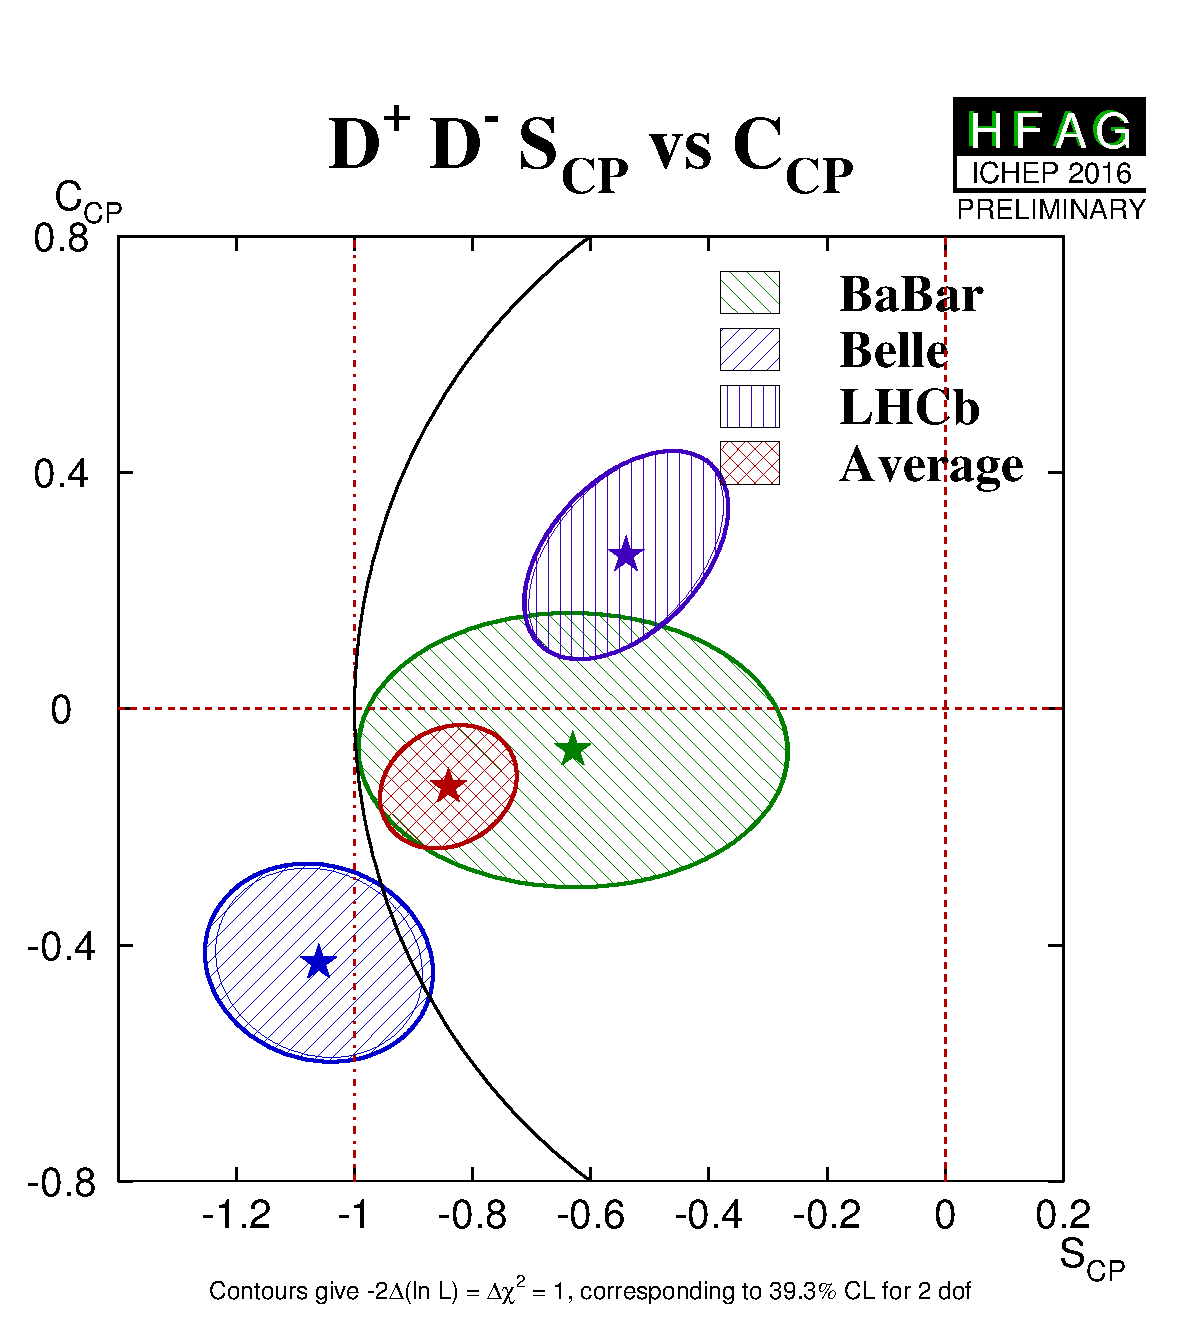
\includegraphics[width=0.5\textwidth]{08-Discussion/figs/D+D-S_CPvsC_CP.png}
\caption{Comparison of \CP observables from \mbox{\BdToDD} decays in (\SDD,
\CDD) plane~\cite{HFAG}. The contours give $-2\Delta(\ln L) = \Delta\chisq =
1$, thereby corresponding to a coverage of \SI{39.3}{\percent} for 2 degrees
of freedom.}
\label{fig:discussion:b2ddcomparison}
\end{figure}
Looking at the uncertainty ellipses it is apparent that the precision of \lhcb
matches the one of \belle, while being significantly better than the one of
\babar. The orientation of the ellipses shows that in the measurements of the
$B$-factories the two \CP observables are determined almost uncorrelated. For
a comparison of the central values it is useful to take into account the arc
defined by the condition $\SDD^2+\CDD^2=1$. It represents the extreme case of
$\lambda_{\Dp\Dm}$ being purely imaginary and delimits the physically allowed
region. The result by \belle~\cite{Rohrken:2012ta} of \SDD = \num{-1.06} and
\CDD = \num{-0.43} lies outside, while the results of
\babar~\cite{Aubert:2008ah}, which are \SDD = \num{-0.63} and \CDD =
\num{-0.07}, as well as the result of \lhcb (see
\cref{eq:b02dd:decaytimefit:cpresults}) are inside.
